% mycsrf 'for beeing included' snippet template
%
% (c) Karsten Reincke, Frankfurt a.M. 2012, ff.
%
% This text is licensed under the Creative Commons Attribution 3.0 Germany
% License (http://creativecommons.org/licenses/by/3.0/de/): Feel free to share
% (to copy, distribute and transmit) or to remix (to adapt) it, if you respect
% how you must attribute the work in the manner specified by the author(s):
% \newline
% In an internet based reuse please link the reused parts to mycsrf.fodina.de
% and mention the original author Karsten Reincke in a suitable manner. In a
% paper-like reuse please insert a short hint to mycsrf.fodina.de and to the
% original author, Karsten Reincke, into your preface. For normal quotations
% please use the scientific standard to cite
%


%% use all entries of the bibliography

\subsection{Elysium ($\bigstar\bigstar\bigstar\bigstar$)}

\parpic(1cm,0.7cm)[r][t]{
\includegraphics[width=1cm]{logos/elysium-300dpi.png}}
\label{Elysium}\acc{Elysium} fungiert als Frontend für \acc{LilyPond}, ohne ein
eigenständiger Editor zu sein. Es wird vielmehr zusammen mit \acc{Eclipse}
genutzt, einer integrierten Entwicklungsumgebung, deren Funktionalität erst über
die Integration von Plugins entsteht. Entwickelt und gepflegt wird diese
IDE\footnote{Integratet Development Environment} von der \acc{Eclipse
Foundation}.\footcite[vgl.][\nopage wp]{Eclipse2018a} Sie bietet die
verschiedensten vorkonfigurierten Pakete an, zusammengestellt für die
unterschiedlichsten Zwecke und ausgelegt auf die gängigsten Betriebssysteme. In
unserem Fall reicht das einfache Standardpaket \enquote{Eclipse IDE for Java
Developers}.\footcite[vgl.][\nopage wp]{Eclipse2018b}

Ein Plugin, das zu installieren in unserem Kontext lohnt, wäre z.B.
\acc{{\TeX}lipse}: es macht \acc{Eclipse} zu einem exzellenten 'Editor' für
\LaTeX-Texte.\footcite[vgl.][\nopage wp]{TeXlipse2019a}

Das für unsere Zwecke entscheidende Plugin ist \acc{Elysium}. Es wird aus
Eclipse heraus vom \enquote{Eclipse-Marketplace} heruntergeladen und
installiert.\footnote{\cite[vgl.][\nopage wp]{Harmath2019a}. Die
Paketbeschreibung sagt, \acc{Elysium} werde unter der \acc{Eclipse Piblic
License} distribuiert, einer offiziellen Open Source Software Lizenz.
( $\rightarrow$ \href{https://opensource.org/licenses/EPL-2.0}
{https://opensource.org/licenses/EPL-2.0}) } Sein Schöpfer nennt seine
Erweiterung die \enquote{LilyPond IDE für Eclipse}.\footcite[vgl.][\nopage
wp]{Harmath2019b} Der Name \acc{Elysium} verweise auf \acc{Eclipse} und
\acc{.ly}, der Extension von LilyPond-Dateien und stehe für eine
\enquote{himmlische} Verbindung: Schließlich sei beides Open-Source-Software,
wobei \enquote{[\ldots] writing complex scores with LilyPond inevitably requires
a more agile, more managed approach than a simple command line and plain text
editor}. Und eben das unterstütze \acc{Eclipse} als bewährte
Entwicklungsumgebung schon von sich aus.\footcite[vgl.][\nopage
wp]{Harmath2019d} Dem entsprechend ist \acc{Elysium} als freie Software
quelloffen unter der \acc{Eclipse Public License} publiziert
worden\footcite[vgl.][\nopage wp]{Harmath2018a}. Das System werde -- wie es
heißt -- in vier Schritten bereitgestellt: Sofern es die eigene Distribution
nicht schon mit sich bringe, installiere man zuerst auf die gewohnte Weise
\acc{LilyPond}, dann \acc{Eclipse} und von da aus das Plugin
\acc{Elysium}.\footcite[vgl.][\nopage wp]{Harmath2019c} Alle Varianten liefen
bei uns problemlos durch.

Von seinen Eigenschaften her ist \acc{Elysium} ein semi-graphischer Editor: man
gibt -- Editor gestützt -- den gewünschten \acc{LilyPond}-Code ein und bei jeder
Sicherung der Quelldatei werden die entsprechende MIDI- und die zugehörige
PDF-Datei kompiliert und angezeigt.\footcite[vgl.][\nopage wp]{Harmath2019e} Auf
diese Weise kann \acc{Elysium} auch mit unser Referenzkadenz II problemlos
umgehen, als \acc{LilyPond}-Frontend sogar inklusive unser kleinen
Zusatzbibliothek:

\begin{center}
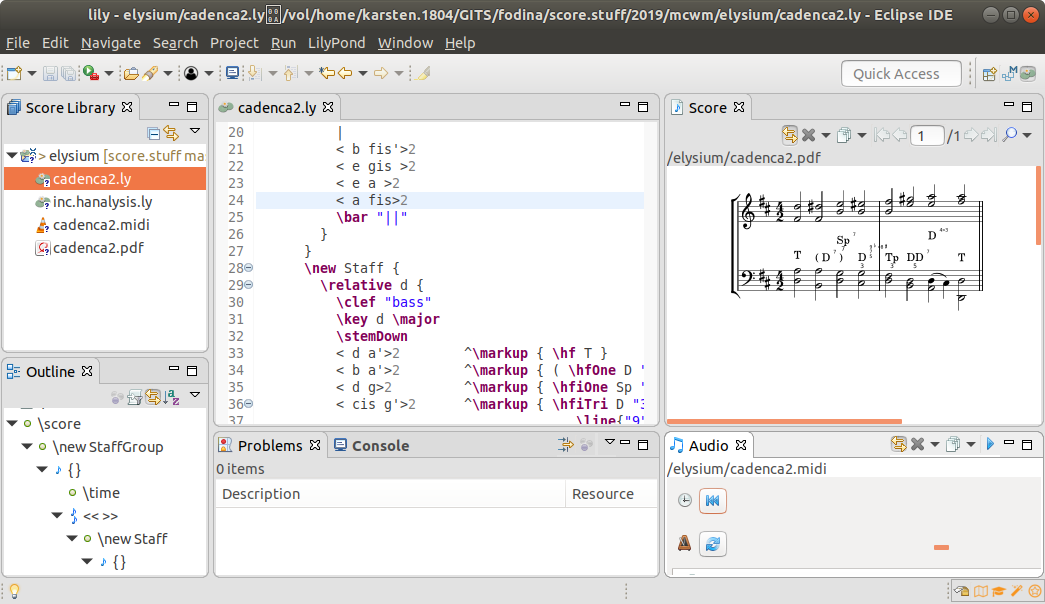
\includegraphics[width=0.9\textwidth]{frontends/elysium/elysium-cadenca2-300dpi.png}
\end{center}

Die \acc{LilyPond}-Perspektive, die das \acc{Elysium}-Plugin mitbringt, enthält
in der oberen Mitte den eigentlichen \acc{LilyPond}-Editor. Er nutzt
Syntaxhighlighting und bietet-- über die Eclipse-Menues -- den bei \acc{Eclipse}
gewohnten Programmiersupport. Links davon findet sich -- entsprechenend -- eine
Liste der Projekte und ihrer Dateien. Und darunter wird die Struktur der Datei
abgebildet, die gerade editiert wird. Auf der rechten oberen Seite erscheint
dann nach jeder Sicherung des eingegebenen Codes der Notentext, der daraus
erzeugt werden kann. Und der rechte untere Bereich bietet einen MIDI-Player, mit
dem man sich seine generierte Musik anhören kann.

Zwei Kleinigkeiten können bei der Nutzung verwirren: 

Zum ersten muss man das 'Noten'-Fenster und das \acc{MIDI}-Player-Fenster an
eine geöffnete Datei 'binden', wenn man den Notentext sehen und hören möchte.
Dazu nutzt man die gelben Pfeile.

Außerdem erwartet \acc{Elysium}, dass in der Projektspalte des Eclipsemenues die
Option 'build automatically' aktiviert ist. Nur dann nämlich generiert
\acc{Elysium} unter Rückgriff auf das installierte \acc{LilyPond}-Backend
automatisch die zurghörige PDF-Datei und -- sofern im Code mit \texttt{MIDI\{\}}
aktiviert -- die entsprechendene MIDI-Datei, die dann im rechten oberen und
unteren Bereich dargestellt werden.

Nun gibt es durchaus Gründe, nicht alle Projekte immer automatisch bilden zu
lassen.\footnote{So schreiben wir z.B. den Text, den Sie gerade lesen, mit
\acc{Elcipse} und \acc{Texlipse}. Gemeinsam wissen wir aber bereits, dass unser
Text nicht standardmäßig prozessiert werden darf, weil ja \texttt{lilypond-book}
immer zuerst ausgeführt werden muss und den eigentlichen \LaTeX-Text erst
generiert.} Will man solche Projekte mit manuellem Anstoß und die
Lilypond-Projekte, die die automatische Abarbeitung fordern, gemeinsam offen
halten, wird man Auto-Build-Funktionen je nach Bedarf an und abschalten müssen
und die Fehlermeldungen souverän ignorieren, von denen man weiß, daß sie
'natürlich' sind. Alternativ kann man natürlich eine weitere Eclipse-Instanz mit
anderem Workspace starten.

Insgesamt erhält man mit \acc{Elysium} eine verlässlich solide Umgebung zur
Entwicklung von \acc{LilyPond} basierten Noten, die insbesondere denjenigen ans
Herz wachsen wird, die eh schon mit \acc{Eclipse} arbeiten.

% this is only inserted to eject fault messages in texlipse
% \bibliography{../bib/literature}
